% Fluxograma da metodologia de pesquisa
% Feito para o ÉguaTeX (eguatex.com.br). Uso livre (CC0 1.0).
%
% Compile e pronto: sai só a figura, em PDF.
% Para pôr no seu trabalho, use o PDF com \includegraphics ou copie
% o bloco tikzpicture para dentro de uma figure e ponha no preâmbulo
% \usepackage{tikz} e \usetikzlibrary{positioning}.
\documentclass[tikz,border=4pt]{standalone}
\usepackage[T1]{fontenc}
\usepackage{lmodern}
\usetikzlibrary{positioning}

\begin{document}
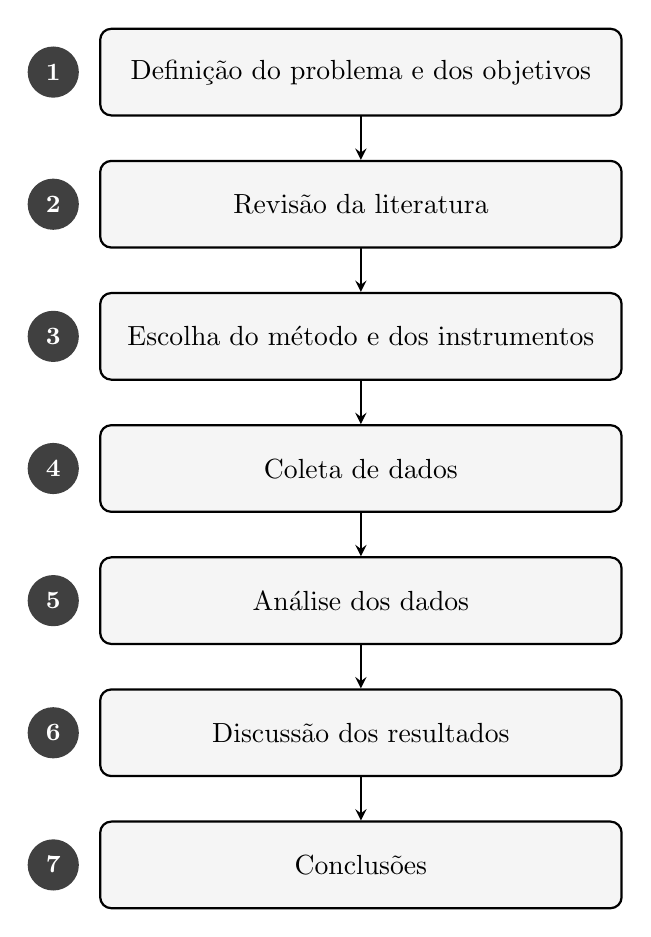
\begin{tikzpicture}[>=stealth, line cap=round, line join=round,
  etapa/.style={draw, line width=0.8pt, rounded corners=4pt, fill=black!4,
    text width=6.2cm, align=center, minimum height=1.1cm, inner sep=6pt},
  numero/.style={circle, fill=black!75, text=white, font=\small\bfseries,
    minimum size=0.65cm, inner sep=0pt},
  seta/.style={->, line width=0.8pt}]

% Mude as etapas aqui: uma por item, separadas por vírgula.
% Use chaves em volta de uma etapa que tenha vírgula no texto.
\def\etapas{
  {Definição do problema e dos objetivos},
  {Revisão da literatura},
  {Escolha do método e dos instrumentos},
  {Coleta de dados},
  {Análise dos dados},
  {Discussão dos resultados},
  {Conclusões}}
\def\distancia{0.55} % espaço entre as caixas, em cm

\foreach \t [count=\i] in \etapas {
  \ifnum\i=1
    \node[etapa] (e\i) {\t};
  \else
    \pgfmathtruncatemacro{\ant}{\i-1}
    \node[etapa, below=\distancia cm of e\ant] (e\i) {\t};
    \draw[seta] (e\ant) -- (e\i);
  \fi
  \node[numero, left=0.25cm of e\i] {\i};
}
\end{tikzpicture}
\end{document}
